\chapter{Introduction to Discrete Probability}

First, let's take care of the word \emph{discrete} vs \emph{discreet}.
They sound exactly the same, but ``discrete'' means ``individually
separate and distinct'' and ``discreet'' means ``careful about what
other people know''.  So you might say, ``You can think of light as a
continuous wave or as a blast of discrete particles.'' And you might
say, ``Please go get the box of doughnuts from the kitchen. Oh, and
there are a lot of hungry people in the house, so be
discreet.''\index{discrete vs. discreet}

When we are talking about probabilities, some problems deal
with discrete quantities like ``What is the probability that I will
throw these three dice and the numbers that roll face up sum to 9?''. There
are also problems that deal with continuous properties like ``What is
the probability that the next bird to fly over my house will weigh
between 97.2 and 98.1 grams ?'' In this module, we are going to focus
on the probability problems that deal with discrete quantities.

Watch Khan Academy's Introduction to Probability at \url{https://youtu.be/uzkc-qNVoOk}.

Let's say that I have a cloth sack filled with 100 marbles; 99 are red
and 1 is white. If I ask you to reach in without looking and pull out
one marble, you will probably pull out a red one. We say that ``There
is a 1 in 100 chance that you would pull out a white marble.'' Or we
can use percentages and say ``There is a 1\% chance that you will pull
out a white marble.'' Or we can use decimals and say ``There is a 0.01
probability that you will pull out a white marble.''
% Bag Diagram
In probability, we often talk about the probability of certain
events. ``Pulling out a white marble'' is an event, and we can give it
a symbol like $W$. Then, in equations we use $p$ to mean ``the
probability of''.  Thus, we can say ``There is a 0.01 probability that
you will pull out a white marble'' which becomes the equation
\begin{equation*}
  p(W) = 0.01
\end{equation*}\index{probability}
% ADD: Make sure functions come before this chapter, connect to functions

\section{The Probability of All Possibilities is 1.0}

We know that you are either going to pull out a red marble or a white marble,
so the probability of a white marble being pulled and the probability
of a red marble being pulled must add up to 100\%. Therefore, the odds of
pulling out a red marble must be 99\% or 0.99. If we let the event ``Pull out a red marble'' be given by the symbol $R$, we can say:
\begin{equation*}
  p(R) = 1.0 - P(W) = 1.0 - 0.01 = 0.99
\end{equation*}

Now, let's say that I make you take a marble from the bag and then
toss a coin. What is the probability that you will pull a white marble
and then get heads on the coin? It is the product of the two
probabilities: $0.01 \times 0.5 = 0.005$, so one-half of a one percent
chance. Do the probabilities still sum to 1?
\begin{itemize}
\item White and Heads = $0.01 \times 0.5 = 0.005$
\item White and Tails = $0.01 \times 0.5 = 0.005$
\item Red and Heads = $0.99 \times 0.5 = 0.495$
\item Red and Tails = $0.99 \times 0.5 = 0.495$
% ADD: add up the values at the end for clarity
\end{itemize}
Yes, the probabilitites of all the possibilities still add to 1.

\section{Independence}

In the last section, I told you that the probability of two events
(``Pulling a red marble from the bag'' and ``Getting tails in a coin
toss'') is the product of the probability of each event: $0.99 \times 0.5 = 0.495$.

This is true if the two events are \textit{independent}, that is the
outcome of one doesn't change the probability of the other.  The
example I gave is independent: It doesn't matter what ball you pull
from the bag, the outcome of the coin toss will always be 50-50.\index{independent}

What are two events that are not independent? The probability that a
person is a professional basketball player and the probability that
someone wears a shoe that is size 13 or larger is \textit{not}
independent. After all, height is an advantage in basketball and most
tall people also have large feet. So if you know someone is a
basketball player, they likely wear large shoes.
% ADD: Correlation for Causeation 
% Weird Correlations Website: https://www.tylervigen.com/spurious-correlations
% KA: https://youtu.be/R-NeYKSEqns

\begin{Exercise}[title={Rolling Dice}, label=rolling-dice]
  If I give you three dice to roll, what is the
  probability that you will roll a 5 on all three dice?
\end{Exercise}
\begin{Answer}[ref=rolling-dice]
  probability of all 5's $ = \frac{1}{6}\times\frac{1}{6}\times\frac{1}{6} = \left(\frac{1}{6}\right)^3 = \frac{1}{216} \approx 0.0046$
  \end{Answer}
    
\begin{Exercise}[title={Flipping Coins}, label=flipping-coins]
  If I give you five coins to flip, what is the
  probability that at least one coin will come up heads?
\end{Exercise}
\begin{Answer}[ref=rolling-dice]
  probability of at least one heads = 1.0 - probability of all tails $ = 1.0 - \left(\frac{1}{2}\right)^5 =1.0 - \frac{1}{32} = \frac{31}{32} = \approx 0.97$ 
  
\includegraphics[width=0.5\textwidth]{coin_prob.png}
\end{Answer}
    
\section{Why 7 is the most likely sum of two dice}

If you roll two dice, the sum will be 2 or 12 or any number in
between. It is very tempting to assume that the likelihood of any of
those numbers is the same. In fact, the probability of a 2 is
$\frac{1}{36} \approx 3\%$ and the probability of a 7 is $\frac{1}{6}
\approx 17\%$. A 7 is six times more likely than a 12! Why?

When you roll the first die, there are six possibilities with equal
probability. When you roll the second die, there are six possibilities
with equal probability. so there are a total of 36 possible events
with equal probabilities: 1 then 1, 1 then 2, 2 then 1, 1 then 3, 3
then 1, etc. Only one of these (1 then 1) adds to 2.  But six of these
sum to 7: 1 then 6, 6 then 1, 2 then 5, 5 then 2, 3 then 4, 4 then
3. So a 7 is six times more likely than a 2.

Here is the complete table:
%Dice Diagram
\begin{tabular}{c| c c c c c c | c | c}
  Sum &     &     &     &     &     &     & Count & Probability \\
  \hline
  2   & 1,1 &     &     &     &     &     &   1    & 1/36 \\
  3   & 1,2 & 2,1 &     &     &     &     &   2    & 1/18 \\
  4   & 1,3 & 2,2 & 3,1 &     &     &     &   3    & 1/12 \\
  5   & 1,4 & 2,3 & 3,2 & 4,1 &     &     &   4    & 1/9 \\
  6   & 1,5 & 2,4 & 3,3 & 4,2 & 5,1 &     &   5    & 5/36 \\
  7   & 1,6 & 2,5 & 3,4 & 4,3 & 5,2 & 6,1 &   6    & 1/6 \\
  8   &     & 2,6 & 3,5 & 4,4 & 5,3 & 6,2 &   5    & 5/36 \\
  9   &     &     & 3,6 & 4,5 & 5,4 & 6,3 &   4    & 1/9 \\
  10  &     &     &     & 4,6 & 5,5 & 6,4 &   3    & 1/22 \\
  11  &     &     &     &     & 5,6 & 6,5 &   2    & 1/18 \\
  12  &     &     &     &     &     & 6,6 &   1    & 1/36
\end{tabular}

When I bumped into this, I was skeptical. I decided to test it, so I
rolled a pair of dice hundreds of times and made a histogram. It was a
tedious and time-consuming task -- just the sort of thing that we make
computers do for us.
% ADD: Define Histogram
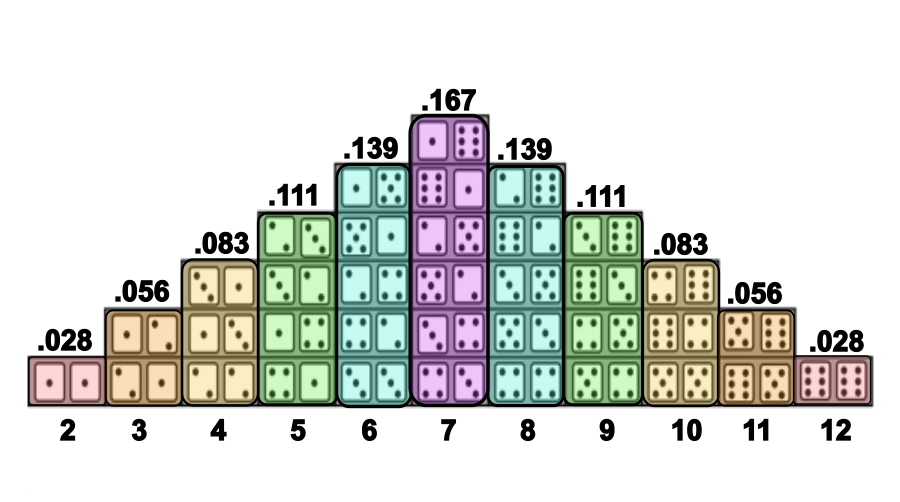
\includegraphics[width=0.5\textwidth]{dice_graph.png}
\section{Random Numbers and Python}

You are going to write a simulation of rolling dice in Python. To do
this, you will need to generate a random sequence of numbers. The
numbers will need to be in the range 1 to 6, and they will need to
appear in the sequence with the same frequency.  We say the sequence
will follow \textit{the uniform distribution}.  That is, the
probability is uniformly distributed among the 6 possibilities.\index{random number generation}

Start python and try a few of the different ways to generate random numbers:
\begin{Verbatim}[commandchars=\\\{\}]
> \textbf{python3}
>>> \textbf{import random}
>>> \textbf{random.random()}  # Generates a random floating point number between 0 and 1
0.6840892758539989
>>> \textbf{randrange(5)}      # Generates an integer in the range 0 - 4
2
>>> \textbf{x = ['Rock', 'Paper', 'Scissors']}
>>> \textbf{random.choice(x)}   # Pick a random entry from the sequence
'Paper'
>>> \textbf{x}
['Rock', 'Paper', 'Scissors'] 
>>> \textbf{random.shuffle(x)}   # Shuffle the order of the sequence
>>> \textbf{x}
['Scissors', 'Paper', 'Rock']
>>> \textbf{a = list(range(30))}
>>> \textbf{a}
[0, 1, 2, 3, 4, 5, 6, 7, 8, 9, 10, 11, 12, 13, 14, 15,
  16, 17, 18, 19, 20, 21, 22, 23, 24, 25, 26, 27, 28, 29, 29]
>>> \textbf{random.sample(a, 10)} # Return 10 randomly chosen items from the sequence
[8, 7, 20, 9, 25, 13, 23, 11, 14, 16]
\end{Verbatim}
% KA: https://www.youtube.com/watch?v=Jua-KWBdzfU
Clearly, Python has a lot of ways to do things that look random. I
should be honest with you at this point: they aren't really
random. The computer that you are using can't generate random
data. Instead, it uses tricks to create data that looks random; we
call this \textit{pseudorandom} data. Good pseudorandom algorithms are
very important for cryptography and data security.

What if you want real random data? Some companies that are using
the decay of radioactive materials to generate real random data. You
can pay to download it. For our purposes, Python's pseudorandom
numbers are quite sufficient.

If we generate two random numbers in the range 1 through 6 and add them together, we
will have simulated rolling a pair of dice. Like this:

\begin{Verbatim}[commandchars=\\\{\}]
>>> \textbf{a = random.randrange(6) + 1}
>>> \textbf{b = random.randrange(6) + 1}
>>> \textbf{a + b}
8
\end{Verbatim}

First, let's write a program that just rolls the dice 100 times and shows the result. Make a file \url{dice.py}:
\begin{Verbatim}
import random

roll_count = 100

for i in range(roll_count):
    a = random.randrange(6) + 1
    b = random.randrange(6) + 1
    roll = a + b
    print(f"Toss {i}: {a} + {b} = {roll}")
\end{Verbatim}

When you run it, you should see something like:
\begin{Verbatim}[commandchars=\\\{\}]
> \textbf{python3 dice.py}
Toss 0: 6 + 6 = 12
Toss 1: 4 + 4 = 8
Toss 2: 4 + 2 = 6
Toss 3: 4 + 6 = 10
Toss 4: 4 + 4 = 8
...
Toss 98: 5 + 2 = 7
Toss 99: 5 + 2 = 7
\end{Verbatim}

Now we want to count occurrences of each possible outcome. Let's use an
array of integers. We will start with an array of zeros. And, for
example, when we roll a 3, we'll add 1 to item 3 in the array. (We can
never roll a zero or a one, so those two entries will always be zero.)
% ADD: Define Array
\begin{Verbatim}[commandchars=\\\{\}]
import random

roll_count = 100

\textbf{# Make an array containing 13 zeros}
\textbf{counts = [0] * 13}

for i in range(roll_count):
    a = random.randrange(6) + 1
    b = random.randrange(6) + 1
    roll = a + b
    print(f"Toss {i}: {a} + {b} = {roll}")

    \textbf{# Increment the count for roll}
    \textbf{counts[roll] += 1}

\textbf{print(f"Counts: {counts}")}
\end{Verbatim}

When you run this, at the end you will see a count for each possible outcome :

\begin{Verbatim}
...
Toss 98: 3 + 2 = 5
Toss 99: 6 + 1 = 7
Counts: [0, 0, 2, 6, 16, 11, 13, 14, 11, 11, 6, 9, 1]
\end{Verbatim}

What was the count that we expected? For example, we expected to see a
2 about once every 36 rolls, right? It might be nice to compare our
count to what we expected. Add a few more lines, and we are going to
increase the number of rolls. You will probably want to delete the
line that prints each roll separately:

\begin{Verbatim}[commandchars=\\\{\}]
import random

\textbf{# Can't ever be 0 or 1}
\textbf{p = [0.0, 0.0, 1/36, 1/18, 1/12, 1/9, 5/36, 1/6, 5/36, 1/9, 1/12, 1/18, 1/36]}
roll_count = 1000

# Make an array containing 13 zeros
counts = [0] * 13

for i in range(roll_count):
    a = random.randrange(6) + 1
    b = random.randrange(6) + 1
    roll = a + b

    # Increment the count for roll
    counts[roll] += 1

\textbf{for i in range(2,13):}
    \textbf{print(f"{i} appeared {counts[i]} times, expected {p[i] * roll_count:.1f}")}
\end{Verbatim}

Now you should see something like:
\begin{Verbatim}
2 appeared 39 times, expected 27.8
3 appeared 55 times, expected 55.6
4 appeared 84 times, expected 83.3
5 appeared 110 times, expected 111.1
6 appeared 160 times, expected 138.9
7 appeared 176 times, expected 166.7
8 appeared 124 times, expected 138.9
9 appeared 93 times, expected 111.1
10 appeared 87 times, expected 83.3
11 appeared 49 times, expected 55.6
12 appeared 23 times, expected 27.8
\end{Verbatim}

Whenever you are dealing with random numbers, the outcome will seldom
be \textit{exactly} what you expected. In this case, however, you should see that your
predictions are pretty close.

\subsection{Making a bar graph}



A bar graph is a nice way to look at quantities like this.  Let's make a bar graph that shows the actual count and the expected count:\index{bar graph!in python}

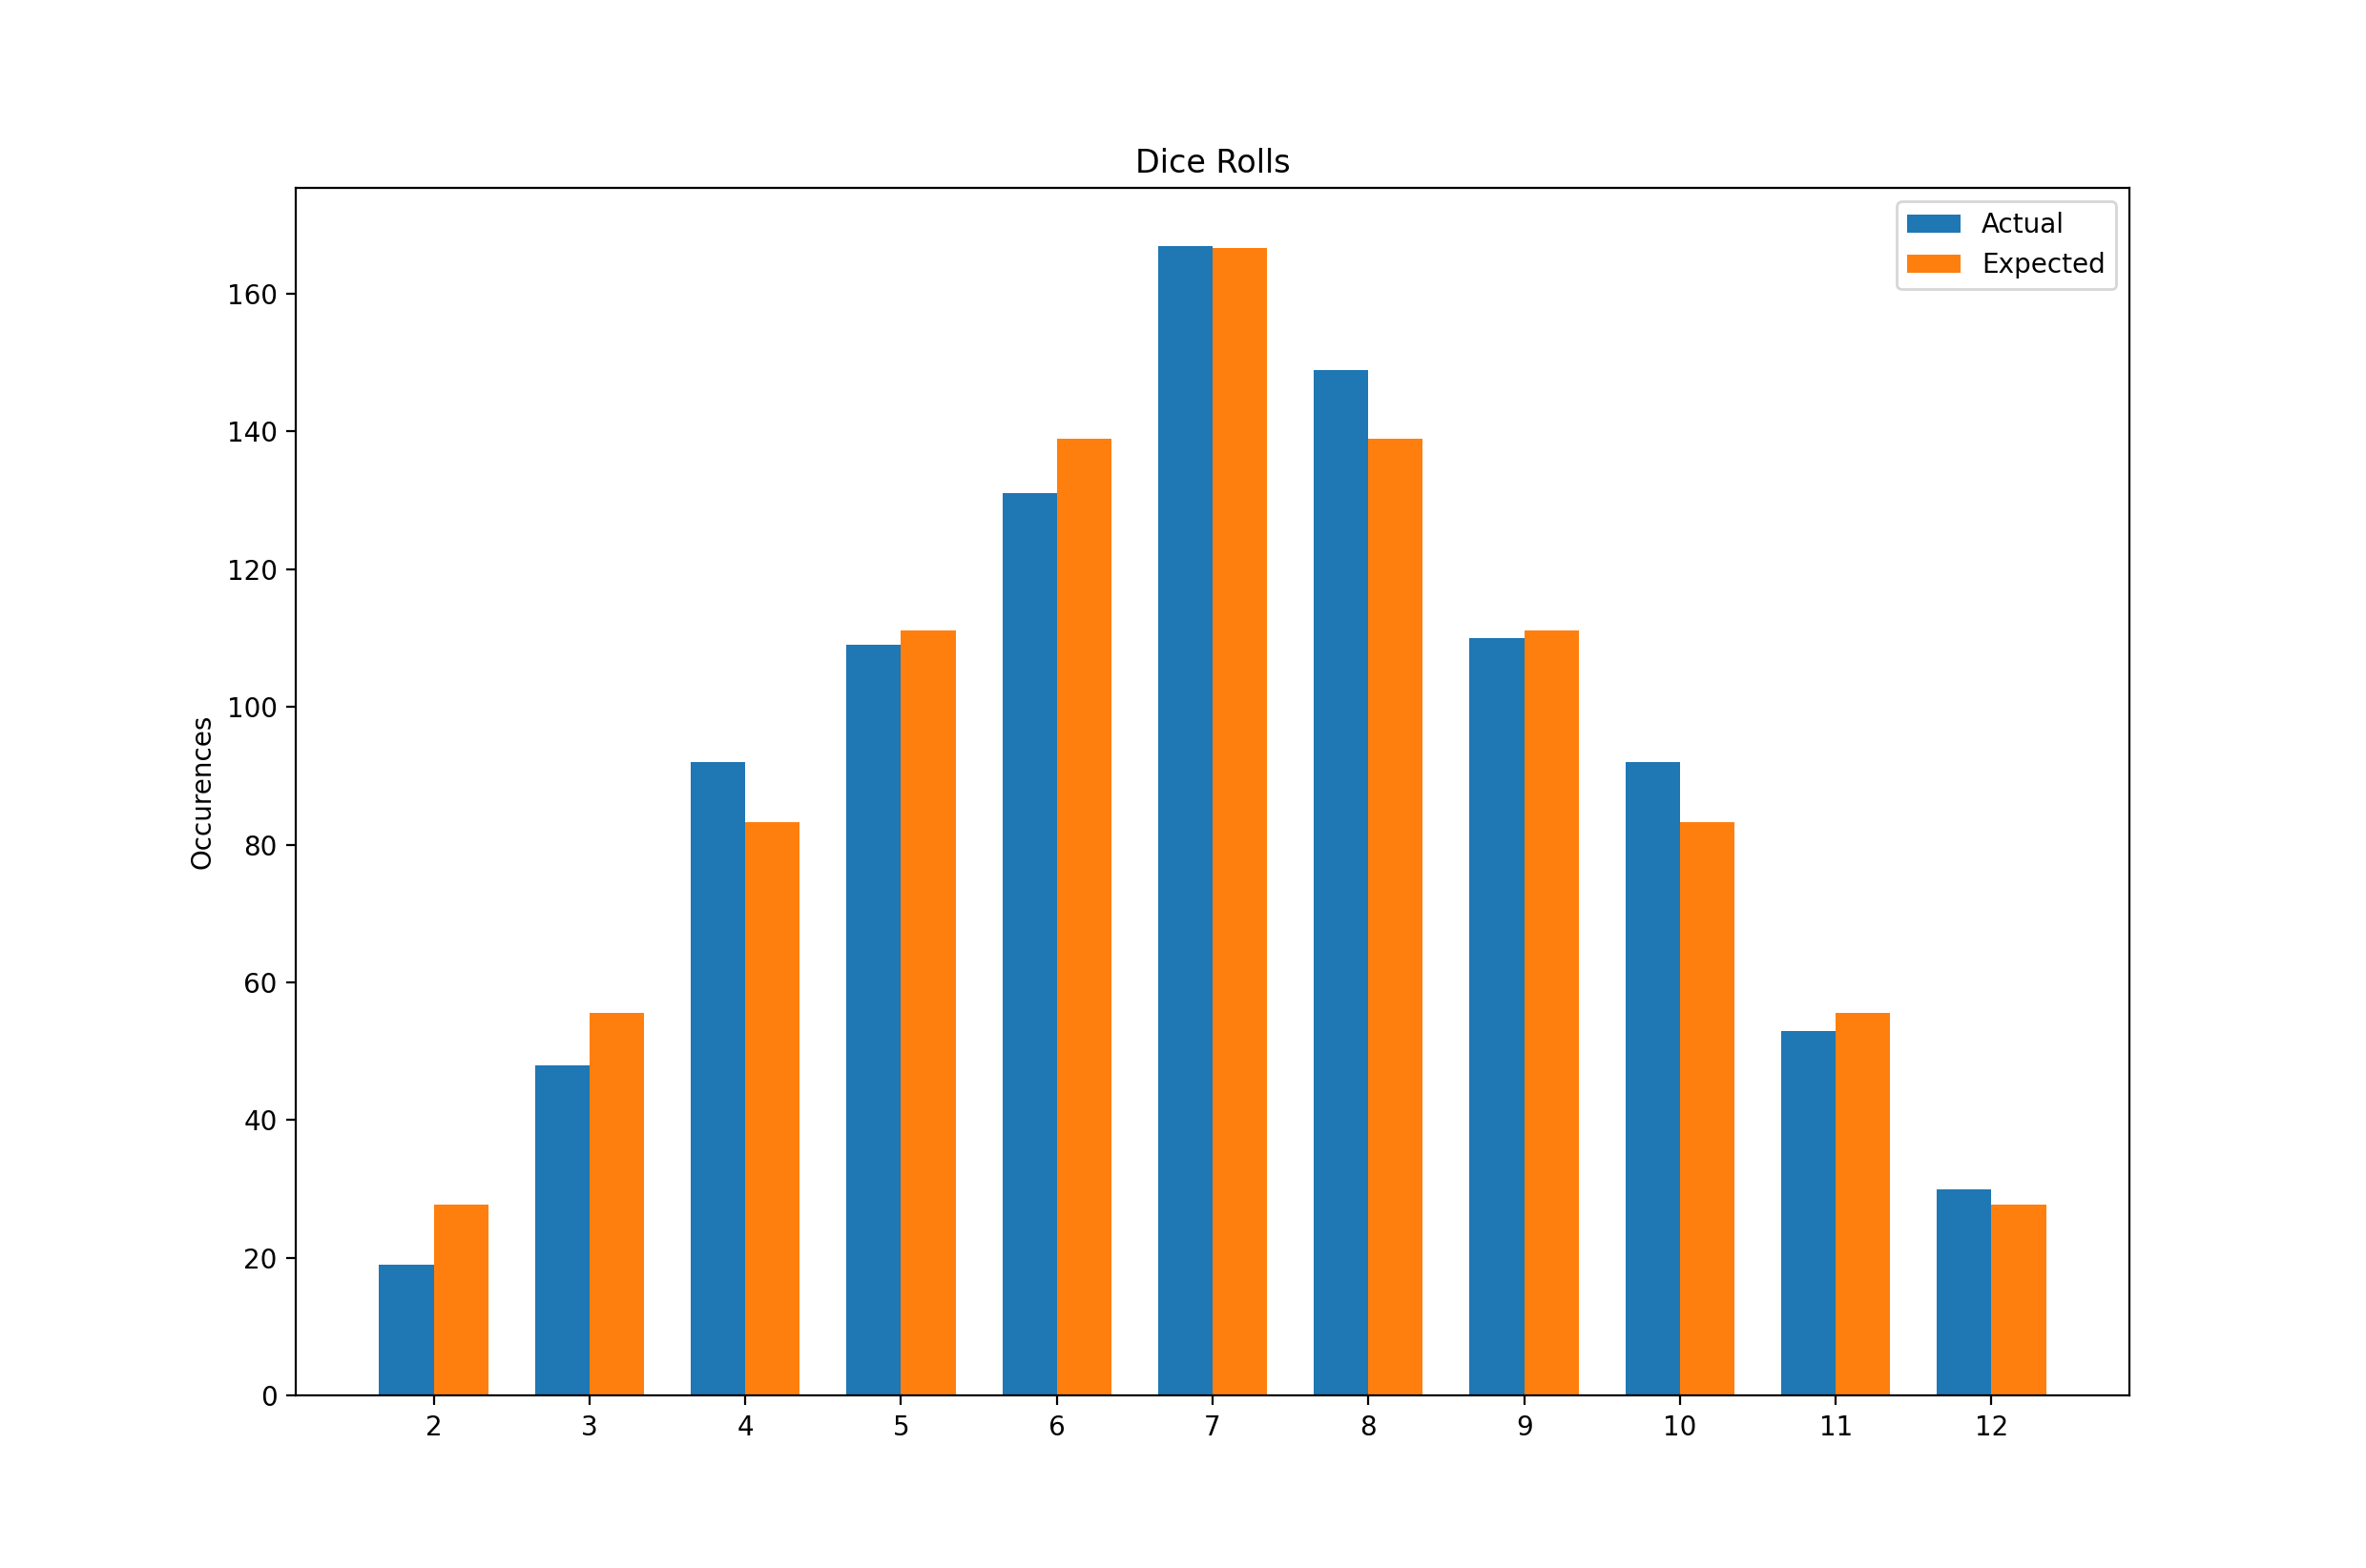
\includegraphics[width= 0.85\textwidth]{dice1.png}

We need to describe the set of rectangles, to do this we will loop through each possible roll (2 - 12) and put data in four lists for each:
% ADD: Define lists
\begin{Verbatim}[commandchars=\\\{\}]
import random
\textbf{import matplotlib.pyplot as plt}

# Can't ever be 0 or 1
p = [0.0, 0.0, 1/36, 1/18, 1/12, 1/9, 5/36, 1/6, 5/36, 1/9, 1/12, 1/18, 1/36]
roll_count = 1000

# Make an array containing 13 zeros
counts = [0] * 13

for i in range(roll_count):
    a = random.randrange(6) + 1
    b = random.randrange(6) + 1
    roll = a + b

    # Increment the count for roll
    counts[roll] += 1

\textbf{# Gather data for bar chart}
\textbf{bar_width = 0.35}
\textbf{expected = []}
\textbf{actual_starts = []}
\textbf{expected_starts = []}
\textbf{labels = []}
\textbf{actual = []}
for i in range(2,13):
    \textbf{expected.append(p[i] * roll_count)}
    \textbf{actual.append(counts[i])}      
    \textbf{actual_starts.append(i - bar_width/2)}
    \textbf{expected_starts.append(i + bar_width/2)}
    \textbf{labels.append(i)}
    
\textbf{fig, ax = plt.subplots()}
    
\textbf{# Create the bars}
\textbf{ax.bar(actual_starts, actual, bar_width, label='Actual')}
\textbf{ax.bar(expected_starts, expected, bar_width, label='Expected')}
\textbf{ax.set_xticks(labels)}

\textbf{# Provide labels}
\textbf{ax.set_ylabel('Occurences')}
\textbf{ax.set_title('Dice Rolls')}
\textbf{ax.legend()}
\textbf{plt.show()}
\end{Verbatim}

% ADD: For extra guideance: https://pythoniseasytolearn.blogspot.com/2019/09/rolling-two-dice.html